\newcommand{\blockIntro}{
\vspace{0.5em}
\begin{center}
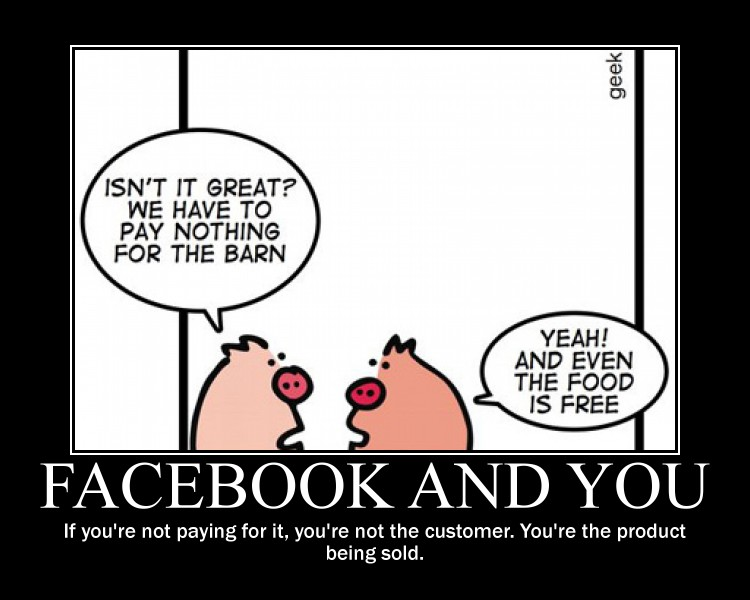
\includegraphics[width=0.6\textwidth]{assets/youre-the-product.jpg}
\end{center}

\textbf{\Large Votre vie privée : un droit fondamental} \\
\vspace{0.5em}
\textit{\Large Constitution Fédérale Suisse, Article 13 :}

\textcolor{darkgray}{\large "Toute personne a droit au respect de sa vie privée et familiale, de son domicile, de sa correspondance et des relations qu'elle établit par la poste et les télécommunications."}

\vspace{1em}

\textbf{\color{c4dtblue}\LARGE Reprenez le contrôle !}
\begin{itemize}
\item{ Des alternatives libres existent}
\item{ Protégez-vous sans sacrifier la simplicité}
\item{ Vos données valent de l'or}
\end{itemize}
}

\newcommand{\blockIntroShort}{
\vspace{0.5em}
\begin{minipage}{0.35\textwidth}
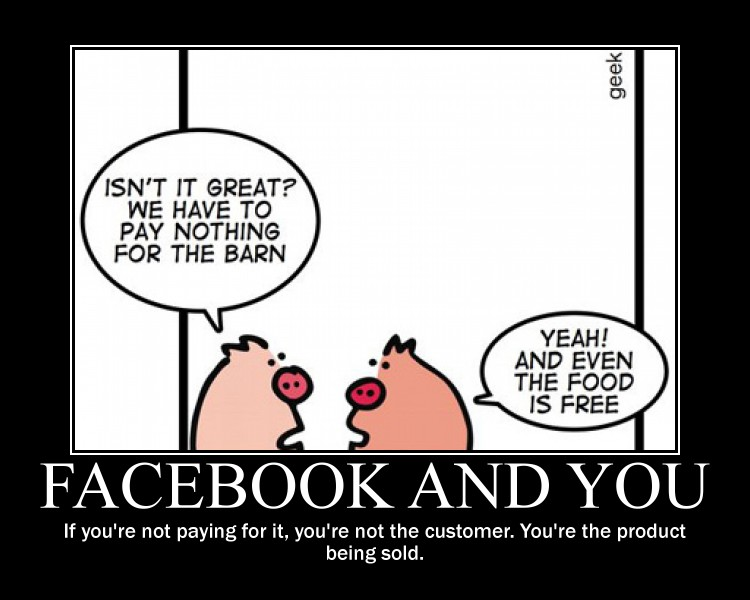
\includegraphics[width=0.9\textwidth]{assets/youre-the-product.jpg}
\end{minipage}
\begin{minipage}{0.6\textwidth}
\textbf{\Large Votre vie privée : un droit fondamental} \\
\vspace{0.5em}
\textit{\Large Constitution Fédérale Suisse, Article 13 :}

\textcolor{darkgray}{\large "Toute personne a droit au respect de sa vie privée et familiale, de son domicile, de sa correspondance et des relations qu'elle établit par la poste et les télécommunications."}

\vspace{1em}

\textbf{\color{c4dtblue}\LARGE Reprenez le contrôle !}
\begin{itemize}
\item{ Des alternatives libres existent}
\item{ Protégez-vous sans sacrifier la simplicité}
\item{ Vos données valent de l'or}
\end{itemize}

\end{minipage}

\vspace{1em}

\blockContactNames[2em]
}

\newcommand{\blockStats}{
\textbf{\color{c4dtblue}\Large E-mail :}
\begin{itemize}
\item{ 251 millions d'emails/minute}
\item{ \textbf{3,4 milliards} d'emails de phishing quotidiens}
\end{itemize}

\vspace{1em}

\textbf{\color{c4dtblue}\Large Surveillance :}
\begin{itemize}
\item{ Profilage comportemental}
\item{ Données vendues aux gouvernements}
\item{ Ciblage publicitaire invasif}
\end{itemize}

\vspace{1em}

\textbf{\color{c4dtblue}\Large Monopolisation :}
\begin{itemize}
\item{ Concentration du pouvoir}
\item{ Contrôle de l'information}
\item{ Restriction des libertés numériques}
\end{itemize}
}

\newcommand{\blockContactNames}[1][0em]{
\begin{minipage}[t]{0.7\linewidth}
  \vspace{#1}
  \textbf{\color{red}Contacts :} \\
  \vspace{2em}
  \small
  \begin{tabular}{ll}
  \\
  C4DT & Carine Dengler (@cdengler@social.epfl.ch) \\
       & Linus Gasser (@ligasser@social.epfl.ch) \\
  GnuGen & Nils Antonovich (@antonovi:gnugen.ch) \\
       & Yaëlle Dutoit (@ydutoit:gnugen.ch) \\
       & Jonas Sulzer (@jonas:violoncello.ch) \\
  DigiGes & https://digitale-gesellschaft.ch \\
  HEIG/VD & Alexis Pinto \\
  \end{tabular}%
\end{minipage}%
\begin{minipage}[t]{0.28\linewidth}
  \begin{flushright}
  \small\textbf{Guide de survie numérique de GnuGen} \\
  \vspace{1em}
  \qrcode[height=0.8\linewidth]{https://gnugen.ch/fr/guides/}
  \footnotesize{gnugen.ch/fr/guides/}
  \end{flushright}
\end{minipage}
}

\newcommand{\blockDiscussion}{
\textbf{\color{red}Qui sommes-nous ?}
\begin{itemize}
\item \textbf{C4DT} - Centre pour la Confiance Numérique
\item \textbf{gnugen} - Promotion du logiciel libre à l'EPFL
\item \textbf{DigiGes} - Partenaire pour la transition numérique
\item \textbf{HEIG/VD} - Haute école d'ingénierie et de gestion
\end{itemize}

\vspace{1em}

\textbf{\color{red}Quelques questions pour commencer :}
\begin{itemize}
\item Qui s'intéresse à mes données? Je n'ai rien à cacher.
\item Comment choisir entre sécurité et confort ?
\item Quel niveau de sécurité me convient ?
\item Pouvez-vous m'aider à installer une application sécurisée ?
\end{itemize}

\vspace{1em}

\blockContactNames
}

\newcommand{\qrspace}{\vspace{1em}}
\newcommand{\qrcodeurl}[3][0.15\linewidth]{
    \centering
    \begin{tikzpicture}
        \node(qrcode){\qrcode[height=\qrcodeheight\linewidth,level=H]{https://#2}};
        \node(overlay){\includegraphics[width=#1]{assets/apps/#3.png}};
    \end{tikzpicture} \\
    \small{#2}
}

\newcommand{\blockCommunication}{
\begin{minipage}{0.7\linewidth}
  \textbf{\color{c4dtblue}X $\rightarrow$ Mastodon}
  \begin{itemize}
    \item Pas d'algorithme manipulateur
    \item Données non vendues aux annonceurs
    \item Contrôle total de votre fil d'actualité
  \end{itemize}
  \vspace{0.5em}
\end{minipage}
\begin{minipage}{0.29\linewidth}
  \qrcodeurl{mastodon.social}{mastodon}
\end{minipage}

\qrspace

\noindent
\colorbox{lightgray}{
  \begin{minipage}{0.27\linewidth}
    \qrcodeurl{signal.org}{signal}
  \end{minipage}%
  \begin{minipage}{0.7\linewidth}
    \hspace{0.5em}
    \textbf{\color{c4dtblue}WhatsApp $\rightarrow$ Signal}
    \begin{itemize}
      \item Métadonnées minimales collectées
      \item Chiffrement vérifié par des experts
      \item Pas de liens avec Meta/Facebook
    \end{itemize}
  \end{minipage}
}

\qrspace

\noindent
\begin{minipage}{0.7\linewidth}
  \textbf{\color{c4dtblue}Slack $\rightarrow$ Matrix}
  \begin{itemize}
    \item Protocole décentralisé et ouvert
    \item Chiffrement bout-à-bout par défaut
    \item Pas d'analyse de vos conversations
  \end{itemize}
\end{minipage}%
\begin{minipage}{0.29\linewidth}
  \qrcodeurl{app.element.io}{matrix}
\end{minipage}
}

\newcommand{\blockOffice}{
\begin{minipage}{0.29\linewidth}
  \qrcodeurl{infomaniak.com/fr/ksuite}{kdrive}
\end{minipage}
\begin{minipage}{0.7\linewidth}
  \textbf{\color{c4dtblue}MS365 $\rightarrow$ K-Drive}
  \begin{itemize}
    \item Données stockées en Suisse (nLPD)
    \item N'utilise pas vos fichiers pour la pub
    \item Peut chiffrer de bout-en-bout
  \end{itemize}
  \vspace{1em}
\end{minipage}%

\qrspace

\noindent
\colorbox{lightgray}{
  \begin{minipage}{0.7\linewidth}
    \textbf{\color{c4dtblue}Outlook $\rightarrow$ Thunderbird}
    \begin{itemize}
      \item Aucune collecte de métadonnées
      \item Open source = transparence totale
      \item Fonctionne avec tous les emails
    \end{itemize}
  \end{minipage}
  \begin{minipage}{0.27\linewidth}
    \qrcodeurl{thunderbird.net}{thunderbird}
  \end{minipage}%
}

\qrspace

\noindent
\begin{minipage}{0.29\linewidth}
  \qrcodeurl{firefox.com}{firefox}
\end{minipage}
\begin{minipage}{0.7\linewidth}
  \textbf{\color{c4dtblue}Chrome $\rightarrow$ Firefox}
  \begin{itemize}
    \item Bloque le tracking par défaut
    \item Moteur indépendant (pas Google)
    \item Extensions anti-pub plus efficaces
  \end{itemize}
\end{minipage}%
}

\newcommand{\blockSecurity}{
\begin{minipage}{0.7\linewidth}
  \textbf{\color{c4dtblue}Gestion de mots de passe}
  \begin{itemize}
    \item Mots de passe uniques et forts
    \item Chiffrement local de vos données
    \item Sécurisé avec un seul mot de passe
  \end{itemize}
  \vspace{0.5em}
\end{minipage}%
\begin{minipage}{0.29\linewidth}
  \qrcodeurl{bitwarden.com}{bitwarden}
\end{minipage}

\qrspace

\noindent
\colorbox{lightgray}{
  \begin{minipage}{0.27\linewidth}
    \qrcodeurl{ublockorigin.com}{ublockorigin}
  \end{minipage}%
  \begin{minipage}{0.7\linewidth}
    \textbf{\color{c4dtblue}Non aux pubs avec uBlock}
    \begin{itemize}
      \item Bloque trackers et publicités invasives
      \item Protection contre sites malveillants
      \item Navigation plus rapide et fluide
    \end{itemize}
  \end{minipage}
}

\qrspace

\noindent
\begin{minipage}{0.7\linewidth}
  \textbf{\color{c4dtblue}Consent-o-matic}
  \begin{itemize}
    \item Refuse automatiquement les cookies
    \item Évite le tracking publicitaire
    \item Enlève les popups
  \end{itemize}
\end{minipage}%
\begin{minipage}{0.29\linewidth}
  \qrcodeurl{consentomatic.au.dk}{consentomatic}
\end{minipage}
}
